\svnInfo $Id$

\section{Node Design}
\label{sec:design}
The \bus defines two {\em physical} types of nodes: member nodes and a control
node. An instantiation of \bus must have one and only one control node and
must have at least one member node (N $\geq$ 1). The maximum number of member
nodes is a function of clock speed, see XXX\_TODO\_XXX for details.

During a transmission, \bus defines three {\em logical} types of nodes:
a transmitting node, a receiving node, and forwarding nodes. During a
transmission, there must be exactly one transmit and one receive node. Any
number (N $\geq$ 0) of forwarding nodes are permitted.

%%%%%%%%%%%%%%%%%%%%%%%%%%%%%%%%%%%%%%%%%%%%%%%%%%%%%%%%%%%%%%%%%%%%%%%%%%%%%%%%
\subsection{Physical Design}
\label{sec:physical}

\begin{figure*}
\begin{center}
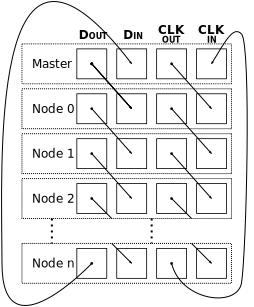
\includegraphics[width=0.5\linewidth]{img/stacked_layers}
\end{center}
\caption{High-level picutre of a \bus design. Member nodes and a control node
are connected in a loop, with a shared {\tt CLK} line running between all
nodes.}
\label{fig:bus}
\end{figure*}

From a package perspective, the physical design of a member and control node
is the same, each must expose a {\tt DIN}, {\tt DOUT}, and {\tt CLK} pin. When
considering a chip to be wirebonded, however, designers must consider that
member nodes will require {\em two} {\tt CLK} pads, as member nodes are
obligated to be able to forward the {\tt CLK} line.

In addition, one (or more?) chip(s) on the bus can add two additional pads to
act as a ``splitter'' node, to allow the interjection of new devices on the
bus. This part of \bus is not yet well-defined.

\subsubsection{Member Nodes}
\label{sec:physical-member}
A member node requires 3 signals:

\begin{itemize}
  \item {\tt DIN} -- Data In
  \item {\tt DOUT} -- Data Out
  \item {\tt CLK} -- Clock {\em (2 Pads)}
\end{itemize}

Most of the time, a member node is in the {\sc forwarding} state. While
forwarding, a member node must amplify and forward signals from the {\tt DIN}
pin to the {\tt DOUT} pin. Designs should attempt to minimize effects on
latency between {\tt DIN} and {\tt DOUT}, in a connected \bus, the maximum
{\tt DOUT} to {\tt DOUT} latency\footnote{
  The amount of time taken to propagate a change in the output of the {\em
  previous} link in the data loop to the output of the next link in the data
  loop. This time includes all of the internal forwarding logic from {\tt DIN}
  to {\tt DOUT}, as well as any pin/wire capacitance that the previous {\tt
  DOUT} must overcome to drive the next link's {\tt DIN}.}
permitted is 10~ns. \bus defines a maximum load capacitance for the {\tt DIN}
pad to be XXX~pF for inter-operability of generalized components\footnote{
  However, the only strict requirement is the 10~ns propogation delay, thus
  careful designers may violate this requirement if necessary.}.

The {\tt CLK} signal is a shared bus. Any physical design must support two
{\tt CLK} wires, one to each neighboring node. On a common chip, this is
simply a shared bus. Chips designed for wirebonding, however, should be sure
to expose two {\tt CLK} pads and electrically connect them on die.

\subsubsection{Control Node}
\label{sec:physical-control}
A control node requires 5 signals:

\begin{itemize}
  \item {\tt DIN} -- Data In
  \item {\tt DOUT} -- Data Out
  \item {\tt CLK} -- Clock
  \item {\tt DSNOOP} -- Data Snoop
  \item {\tt MODE} -- Mode select
\end{itemize}

The control node is responsible for the generation of the {\tt CLK} signal.
Thus, unlike member nodes in a wire-bonded system, the control node has a
minimum of one {\tt CLK} pad instead of two.

The exact functionality of the {\tt DSNOOP} and {\tt MODE} pins is not yet
defined.

\subsubsection{Bus Connections}
\label{sec:physical-bus}
\begin{itemize}
  \item {\tt CLK}
  \begin{itemize}
    \item The clock pins should be wired together to form an electrically
      connected bus.
    \item The only {\tt CLK} driver is on the control node. Designs should
      consider the drive strength of the control node, overall bus
      capacitance, etc.
    \item TODO: Define minimum slew rate, per-chip max {\tt CLK} capacitance,
      etc
  \end{itemize}
  \item {\tt DIN}, {\tt DOUT}
  \begin{itemize}
    \item The data lines should be connected in a round-robin fashion, the
      {\tt DOUT} of one chip connected to the {\tt DIN} of the next.
    \item The connection of data lines must form a loop when connected
      correctly (e.g.~Figure~\ref{fig:bus}).
    \item There are no requirements for the placement of nodes in the data
      loop, but the ordering will have an impact on bus arbitration. See
      Section~\ref{sec:protocol-arbitration} for more details.
  \end{itemize}
  A \bus must have a minimum of two nodes (one control node and one
  member node). Single chips that are not connected to a bus should tie
  {\tt CLK} and {\tt DIN} high and leave {\tt DOUT} floating.
\end{itemize}



%%%%%%%%%%%%%%%%%%%%%%%%%%%%%%%%%%%%%%%%%%%%%%%%%%%%%%%%%%%%%%%%%%%%%%%%%%%%%%%%
\subsection{Logical Design}
\label{sec:logical}

There are three {\em logical} types of \bus nodes: transmitting, receiving,
and forwarding. \bus can be considered `multi-master', any node is capable of
transmitting to any other node. The control node adopts these same three
personalities, but its behavoir differs slightly during
arbitration~(\ref{sec:protocol-arbitration}) and
Bus~Reset~(\ref{sec:protocol-reset}).

\begin{figure}[h]
  \begin{minipage}[b]{.48\linewidth}
    \centering
    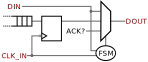
\includegraphics[width=\textwidth]{img/logical}
    \caption{A sketch of the logical model of a node. The Finite State Machine
  selects between the three modes a node can be in. Top: {\em forwarding}, Mid:
  {\em transmitting}, Bot: {\em acknowledging}. This model omits some of the
  subtleties of arbitration, see~\ref{sec:state-arbitrate} for details.
    }
    \label{fig:logical}
  \end{minipage}
  \hspace{1 em}
  \begin{minipage}[b]{.48\linewidth}
    \centering
    %\includegraphics[width=\textwidth]{img/states}
    %\caption{A FSM that needs to be drawn in something other than dot.}
    \label{fig:states}
  \end{minipage}
\end{figure}

\begin{figure}[h]
  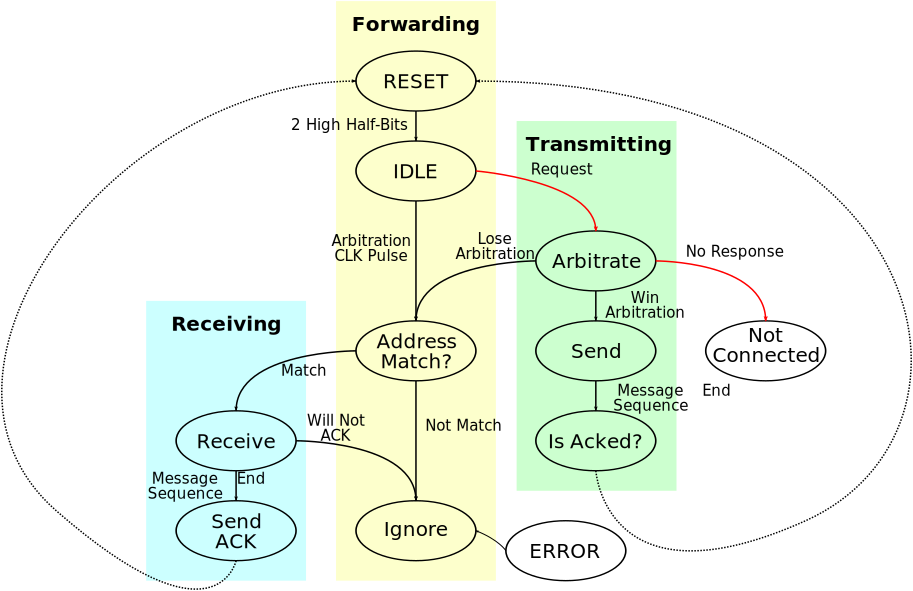
\includegraphics[width=\linewidth]{img/fsm_diagram}
  \caption{A FSM describing the logical behavoir of \bus nodes. All
transitions except \textsc{Idle}$\rightarrow$\textsc{Arbitrate} occur on
rising {\tt CLK} edge. Not shown are implicit arrows from every state returning to
\textsc{reset} any time a Bus~Reset event occurs.}
\end{figure}

\subsubsection{Forwarding}
Forwarding is the most common state for all \bus nodes.  Observe in
Figure~\ref{fig:logical} the very simple, short logic path from {\tt DIN} to
{\tt DOUT}. Nodes are obligated to forward data in less than 10~ns.

\paragraph{Forwarding.\textsc{reset}}
Any time a Bus~Reset event occurs, nodes return to {\sc reset}. After four
clock pulses, nodes transition to {\sc idle}. Note that it is both common and
expected (Message~End~Sequence~$\rightarrow$~Message~Acknowledgement) to loop
Bus~Reset events, transitioning from {\sc reset} to {\sc reset}.

\paragraph{Forwarding.\textsc{Idle}}
This is the rest/idle state for \bus nodes.

\medskip
\noindent
{\em Control Node Exception:} In \textsc{idle}, the control node does not
forward {\tt DIN} to {\tt DOUT}.

\paragraph{Forwarding.\textsc{Address\_Match}}
At the start of a new transmission, a forwarding node should monitor the {\tt
DIN} line to see if it is the target for this transmission. If a node matches
its address, it promotes itself from forwarding to receiving. After the first
mis-matched bit a forwarding node transitions to the {\sc ignore} state for
the rest of the transaction.

\paragraph{Forwarding.\textsc{Ignore}}
In {\sc ignore} nodes simply forward data. Nodes remain in this state until a
Bus~Reset event occurs.

\subsubsection{Transmitting}

\paragraph{Transmitting.{\sc arbitrate}}
\label{sec:state-arbitrate}
A node initiates a transmission by pulling its {\tt DOUT} line low. A node may
only attempt to initiate a transmission while the bus is idle. Care must be
taken in detecting the bus idle state when requesting to transmit, in
particular a node requesting to transmit must ensure that the {\tt CLK} line
is still high, it is not sufficient to rely on the local state machine still
being in the {\sc idle} state\footnote{To envision the case defended against
here, picture a tall stack of nodes, where the bottom node requests the bus.
The control node pulls {\tt CLK} low in response. Shortly before the control
node pulls {\tt CLK} high, a node at the top of the stack (still in the {\sc
idle} state) elects to transmit. There is not enough time for his {\tt DOUT}
to propagate to the bottom node, however, thus when {\tt CLK} goes high, both
the bottom and top nodes believe they have won the arbitration.}.

The {\sc arbitrate} state is left when the {\tt CLK} line is pulled high by
the control node. If a member node's {\tt DIN} is high on the rising clock
edge, it has won arbitration. A node that loses arbitration should begin
listening to see if it is the destination node. If the {\tt CLK} line never
goes high---where never is defined as four times the minimum clock speed of
\bus\footnote{TBD}---the node should consider itself as disconnected.

\medskip
\noindent
{\em Control Node Exception:} The control node always wins arbitration. Note
that when this occurs, the control node's {\tt DIN} will be low.

\medskip
\noindent
{\em Control Node Exception:} If a control node pulls its {\tt DOUT} line low
and its {\tt DIN} line never goes low, it should be considered
{\sc Not\_Connected}.

\paragraph{Transmitting.{\sc send}}
During {\sc send}, a transmitting node pushes bits onto the bus as described
in~\ref{sec:protocol-transmission}. Note that even a transmitting node still
must listen on {\tt DIN} for a Bus~Reset sequence, as the control node is
permitted to cancel a running transmission.

A transmitting node completes its transmission by sending the
Message~End~Sequence~(\ref{sec:protocol-end}).

\paragraph{Transmitting.{\sc Is\_acked?}}
After completing its transmission, a node listens for an immediate
acknowledgement. Regardless of whether the transmission is acknowledged, this
ends the node's ownership of the bus. If a message is not acknowledged, the
transmitter must again negotiate access to the bus.

\subsubsection{Receiving}

\paragraph{Receiving.{\sc Recieve}}
A receiving node is also obligated to forward data along the bus. In the
sketch shown in Figure~\ref{fig:logical}, during the receiving process, a
receiving node remains in pass-thru mode until the Message~End~Sequence.

\paragraph{Receiving.{\sc Send\_Acknowledge}}
A receiver must acknowledge the successful receipt of a transmission. If a
receiver wishes to NAK a transmission, it simply does nothing and allows the
Message~End~Sequence Bus~Reset to occur.

\subsubsection{Non-Standard States}

\paragraph{\sc Not\_Connected}
A robust implementation should include detection of some kind for an attempt
to utilize the bus when the node is not actually connected to a bus (so that
it may report failure). After a node pulls its {\tt DOUT} low there is a
maximum possible $t_{long}$ of XXX\_TODO\_XXX before a control node must pull
{\tt CLK} low in response. If {\tt CLK} is not pulled low, the node should
consider itself disconnected and report failure to send as appropriate.

\paragraph{\sc Async\_reset}
If a node (other than the receiving node) elects to issue a Bus~Reset in the
middle of a transmission, it should enter the {\sc async\_reset} state. The
primary purpose for this state is to properly transition into {\sc
false\_mes\_fix} if necessary, see the note in~\ref{sec:protocol-reset} for
details.

\paragraph{\sc False\_mes\_fix}
When a non-receiving node issues a Bus~Reset event, it is possible that in the
process it inadvertently issues a Message~End~Sequence. This occurs when a
node issuing a reset elects to reset when the currently transmitting bit is a
{\tt 0}. To correct this, the resetting node must distinguish for the
receiving node that this is actually a Bus~Reset event by driving an
additional {\tt 0} on the bus (details:~\ref{sec:protocol-reset}).
